\ylDisplay{Gravitatsioonilääts} % Ülesande nimi
{Mihkel Kree} % Autor
{piirkonnavoor} % Voor
{2007} % Aasta
{G 10} % Ülesande nr.
{8} % Raskustase
{
% Teema: Geomeetriline-optika
\ifStatement
Üldrelatiivsusteooria ennustab, et mustast august möödumisel kaldub valguskiir gravitatsiooni tõttu kõrvale oma esialgsest liikumissuunast nurga $\varphi = 4GM/c^2r$ võrra, kus $M$ on musta augu mass ning $r$ trajektoori lähima punkti kaugus selleni. Sattugu must auk täpselt vaatleja ja tähe vahele, nii et kaugus vaatlejast musta auguni on $L_1$ ning mustast august täheni $L_2$. Missugune on tähe kujutis vaatleja jaoks (põhjendage oma vastust kiirte käigu visandi abil) ning kui suur on kujutise nurkläbimõõt? Kuna vaatlejani jõudvate kiirte jaoks on $r$ palju väiksem tähe kaugusest, võib kasutada väikeste nurkade lähendust $\sin \alpha \approx \tan \alpha \approx \alpha$.
\fi


\ifHint
Kuna silmani jõudvate kiirte jaoks kehtib $r \ll L$ ning trajektoori kõverdumine toimub musta augu lähiümbruses, võib vaadelda kiire teekonda lihtsustatult: kiire liikumine musta auguni, hetkeline nurga muutus musta augu juures ning edasi sirge tee vaatlejani.
\fi


\ifSolution
Tähest väljunud kiired kõverduvad musta augu lähiümbruses (vt joonist). 

\begin{center}
	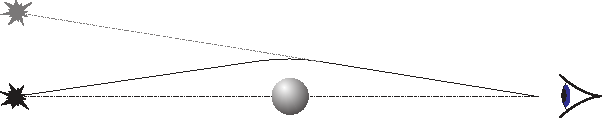
\includegraphics[width=0.9\textwidth]{2007-v2g-10-lah1}
\end{center}

Kujutise konstrueerimisel aga eeldatakse, et kiired on kogu tee otse liikunud. Et kiired jõuavad vaatlejani kõikjalt ümber musta augu, on kujutiseks ringjoon (eeldusel, et täht on punkt).

Et silmani jõudvate kiirte jaoks kehtib $r \ll L$ ning trajektoori kõverdumine toimub tähe lähiümbruses, võib vaadelda kiire teekonda lihtsustatult: sirge liikumine musta auguni, hetkeline nurga muutus musta augu juures ning edasi sirge tee vaatlejani (vt joonist). Joonisel arusaadavalt on vertikaalskaala võrreldes horisontaalskaalaga oluliselt välja venitatud.

Järgnevalt leiame tähe nurkdiameetri. Lihtsast geomeetriast järeldub, et $\alpha + \beta = \varphi$. Kaugused on suured ning nurgad väikesed, seega võime kasutada ligikaudseid valemeid $\alpha = r/L_1$ ja $\beta = r/L_2$. Niisiis

\begin{center}
	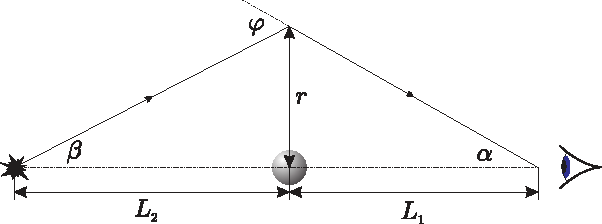
\includegraphics[width=0.9\textwidth]{2007-v2g-10-lah2}
\end{center}

\begin{center}
	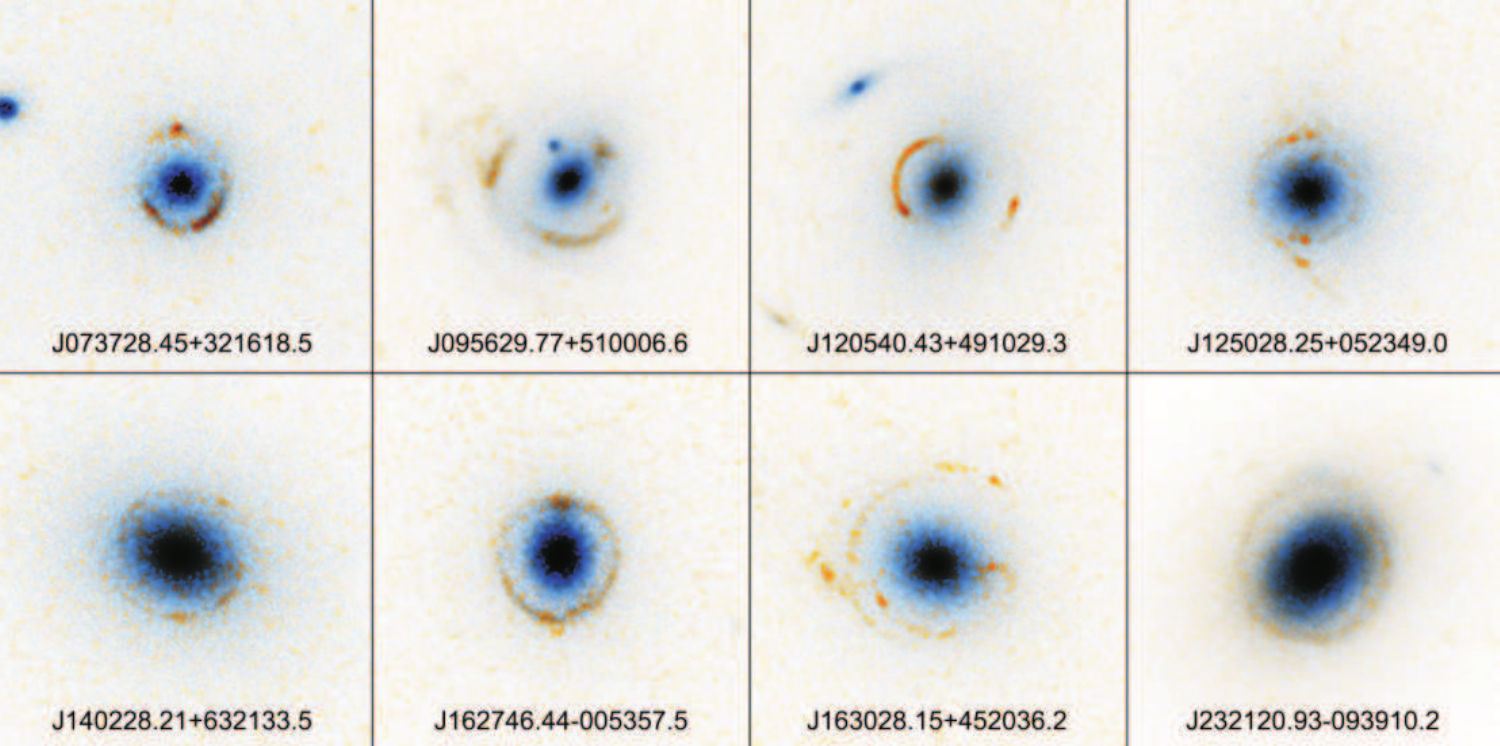
\includegraphics[width=\textwidth]{2007-v2g-10-lah3}
\end{center}

\[
\frac{r}{L_{1}}+\frac{r}{L_{2}}=\frac{4 G M}{c^{2} r} \Rightarrow r=\sqrt{\frac{4 G M L_{1} L_{2}}{c^{2}\left(L_{1}+L_{2}\right)}}.
\]
Tähe kujutise nurkdiameeter on
\[
\gamma=\frac{2 r}{L_{1}}=\sqrt{\frac{4 G M L_{2}}{c^{2} L_{1}\left(L_{1}+L_{2}\right)}}.
\]
\fi
}